\documentclass[11pt]{article}

\usepackage[a4paper,margin=1in]{geometry}
\usepackage[T1]{fontenc}
\usepackage[utf8]{inputenc}
\usepackage{lmodern}
\usepackage{amsmath,amssymb,bm}
\usepackage{booktabs}
\usepackage{array}
\usepackage{tabularx}
\usepackage{graphicx}
\usepackage{xcolor}
\usepackage{microtype}
\usepackage{cite}
\usepackage[hidelinks]{hyperref}
\usepackage{authblk}
\usepackage{float}
\usepackage[section,above,below]{placeins}
\usepackage[font=small,labelfont=bf]{caption}
\captionsetup[figure]{name=Figure,labelsep=colon}
\usepackage{fancyhdr}
\pagestyle{fancy}
\fancyhf{}
\cfoot{\thepage}
\renewcommand{\headrulewidth}{0pt}
\renewcommand{\footrulewidth}{0pt}
\fancypagestyle{plain}{
  \fancyhf{}
  \cfoot{\thepage}
  \renewcommand{\headrulewidth}{0pt}
  \renewcommand{\footrulewidth}{0pt}
}

\graphicspath{{figures/}}
\hypersetup{
  pdftitle={Supplementary Material: A Geometric Criterion for Sway and Rocking in Inclined Pile Groups},
  hypertexnames=false
}
\setlength{\emergencystretch}{3em}
\renewcommand{\topfraction}{0.85}
\renewcommand{\bottomfraction}{0.80}
\renewcommand{\textfraction}{0.07}
\renewcommand{\floatpagefraction}{0.70}

\newcolumntype{L}{>{\raggedright\arraybackslash}X}
\newcommand{\degr}{$^{\circ}$}

% Numbering: Section S1, Figure S1, Table S1
\renewcommand{\thesection}{S\arabic{section}}
\renewcommand{\thefigure}{S\arabic{figure}}
\renewcommand{\thetable}{S\arabic{table}}

\title{Supplementary Material\\[4pt]
\large A Geometric Criterion for Sway and Rocking in Inclined Pile Groups, with Field Identification of an Offshore Wind Turbine Foundation}
\author{Nguyen Hoang Bui, Thi Cam Nhung Nguyen, Huu-Quyet Nguyen, Chung Truong Thanh, Hung Nguyen-Dang, Jos\'e C. Matos}
\date{}

\begin{document}
\maketitle

\noindent This document collects the material that supports the main paper but
is not needed to follow its argument: the quality of the raw records, the
simulation that sets the threshold of the first check, the complete list of
identified poles, the test of the processing settings, the search for a tower
mode, and the setup-by-setup comparison of the two campaigns. Section, figure and
table numbers without the prefix S refer to the main paper.

% =====================================================================
\section{Quality of the raw records}
\label{sec:s-quality}

Table~\ref{tab:records} gives the statistics of the raw records of the seven
setups, and Figure~\ref{fig:quality} shows a typical record of campaign 2. At
one moment a single channel jumps far above its normal level while the others
stay quiet. The event rings briefly at a high frequency, as a sensor mounting
does when it is struck, and is most likely a knock on or near that sensor
rather than a motion of the cap, which would appear on every channel. Most of
the signal energy lies in the mains harmonics between 50 and 200~Hz, and less
than 1\,\% in the structural band below 5~Hz. The records of campaign 1 are
less steady still: the signal level of some channels changes strongly during a
record, and some channels are much weaker than others. Only the three-channel
setup of campaign 1 is close to steady broadband noise.

\begin{table}[htbp]
\centering
\caption{Measurement setups and raw-record statistics. \emph{Ch.} is the number of channels and \emph{Min.} the record length in minutes. \emph{Peak}/$\sigma$ is
the largest absolute sample of any channel divided by that channel's standard
deviation; \emph{Kurt.} the largest channel kurtosis; $N_{>8\sigma}$ the largest number of samples of one channel beyond $8\sigma$; \emph{Drift} the ratio of largest to smallest channel RMS over
ten equal segments; \emph{Spread} the ratio of the largest to the smallest
channel standard deviation within a setup. The largest value of each column is in bold}
\label{tab:records}
\begin{tabular}{@{}llrrrrrrrr@{}}
\toprule
Camp. & Setup & Ch. & Samples & Min. & Peak/$\sigma$ & Kurt. & $N_{>8\sigma}$ & Drift & Spread \\
\midrule
1 & Vertical       & 5 & 2\,535\,936 & 25.6 & 133 & 562  & 2238 & 3.2 & 6.1 \\
1 & Lateral 1      & 5 & 1\,523\,873 & 15.4 & 25  & 54   & \textbf{3131} & 12.9 & \textbf{47.0} \\
1 & Lateral 2      & 5 & 1\,385\,189 & 14.0 & 50  & 1812 & 1063 & \textbf{112} & 9.2 \\
1 & Three-channel  & 3 & 1\,545\,336 & 15.6 & 10  & 4    & 9    & 1.5 & 33.7 \\
2 & Lateral        & 6 & \phantom{0}906\,399 & \phantom{0}9.1 & \textbf{139} & \textbf{3883} & 724 & 4.7 & 11.5 \\
2 & Vertical d1    & 6 & 1\,875\,536 & 18.9 & 69  & 95   & 695  & 4.4 & 4.1 \\
2 & Vertical d2ke  & 6 & 2\,260\,219 & 22.8 & 67  & 88   & 2564 & 4.3 & 4.2 \\
\bottomrule
\end{tabular}
\end{table}

\begin{figure}[htbp]
\centering
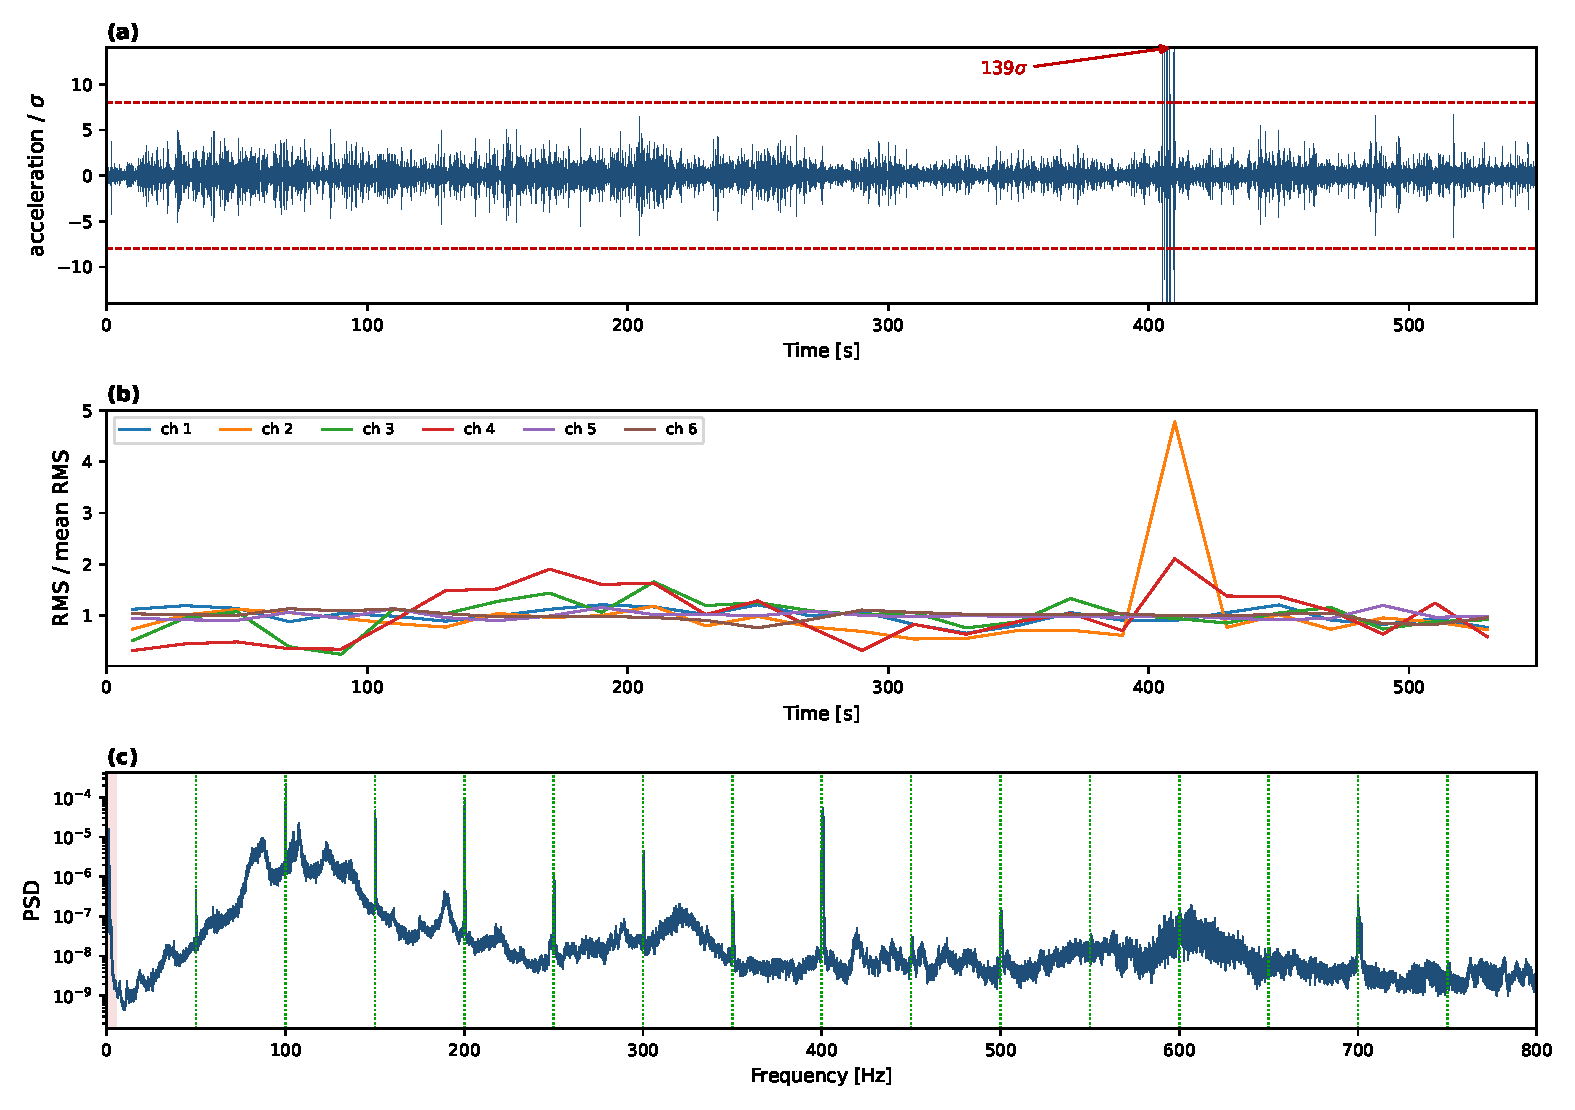
\includegraphics[width=0.95\linewidth]{fig04_record_quality}
\caption{One record of campaign 2. (a) Time history of the channel with the largest event (arrow), in units of its standard deviation. (b) Running RMS of every channel; the event appears on one channel only. (c) Spectrum averaged over the channels, with multiples of 50~Hz dotted and the structural band shaded}
\label{fig:quality}
\end{figure}

% =====================================================================
\section{Threshold of the effective channel count}
\label{sec:s-neff}

The first check of Section~4.2 rejects a pole whose effective channel count
$N_{\mathrm{eff}} = (\sum|\phi|^2)^2 / \sum|\phi|^4$ is below 1.25. The
threshold was set by simulation. Two cases were generated with the sampling
rate, the record length of the shortest record (28\,000 samples at 51.61~Hz)
and the spectral resolution of the measurements:

\begin{itemize}
\item \emph{local response}: a narrow-band signal at 1.2~Hz with 2\,\% damping
on one channel only, and independent white noise on every channel;
\item \emph{mode of the cap}: the same signal shared by all five or six
channels with the measured shape of the low band, in which opposite corners
move in antiphase and the centre hardly moves, again with independent noise
on every channel.
\end{itemize}

Each case was repeated 400 times, at signal-to-noise ratios of 3 and 10, and
$N_{\mathrm{eff}}$ was computed exactly as for the measurements, from the first
singular vector of the cross-power spectral density matrix at the peak of the
1.0--1.4~Hz band. A signal on a single channel never gave more than 1.00. A
mode shared by the channels gave a median of 1.55 with five channels and 1.77
with six, and 1.5 or more in 95\,\% of the trials, at either signal-to-noise
ratio. The threshold of 1.25 was placed between the two cases; it is a convention, not an optimised bound. The shape used for the shared mode is the measured shape of the vertical setup of campaign 1, so the simulation tests the effect of noise and level, not of shape. In the measurements $N_{\mathrm{eff}}$ is evaluated once for each setup and band, at the spectral peak of the band, not for each pole.

Two sensitivities were also examined. A difference of gain of up to 3\,\%
between channels, the largest difference between the sensitivities listed in
the processing log, changes $N_{\mathrm{eff}}$ of the shared mode by at most
4\,\% (1.49 to 1.62), which leaves it well above the threshold. Channel levels
that differ by up to a factor of ten are more harmful: the
count of a real mode then fell below 1.25 in 21\,\% of the trials, so the
check can wrongly reject a real mode in such a record. In the same trials a
local response never exceeded 1.01, so the check did not accept one. With three
channels the two cases cannot be told apart, and the threshold is not applied
to the three-channel setup.

% =====================================================================
\section{Complete list of identified poles}
\label{sec:s-poles}

Table~\ref{tab:poles} lists every pole returned below 25~Hz, by setup, with the spectral peak of frequency domain decomposition (FDD) nearest to the low-band poles. Poles with damping outside 0.1 to 15\,\% are discarded by the identification and do not appear. Table~\ref{tab:phase} gives the phase between opposite corners of the instrumented frame at the peak of the low band, which underlies Figure~7 of the main paper.

\begin{table}[htbp]
\centering
\caption{Poles returned by the identification, by setup; frequency in Hz with damping ratio in per cent
in parentheses}
\label{tab:poles}
\small
\begin{tabularx}{\linewidth}{@{}cl>{\hsize=0.8\hsize}Ll>{\hsize=1.2\hsize}L@{}}
\toprule
Camp. & Setup & Poles below 3~Hz & FDD peak & Poles from 3 to 25~Hz \\
\midrule
1 & Vertical & 1.174 (4.74) & 1.134 & 18.132 (0.70), 18.565 (0.68), 19.077 (0.58), 19.466 (0.59), 19.920 (1.30) \\
1 & Lateral 1 & 1.226 (3.43), 1.254 (2.77), 1.731 (5.49) & 1.248 & 21.920 (0.40), 22.751 (0.51), 23.754 (0.30) \\
1 & Lateral 2 & 1.322 (2.71) & none & 21.574 (5.95), 22.813 (1.25), 23.173 (0.59) \\
1 & Three-channel & 1.238 (3.01), 1.331 (4.39), 1.726 (5.35) & 1.235, 1.311 & 14.438 (1.42), 14.996 (0.97) \\
2 & Lateral & 1.052 (2.69), 1.215 (1.93), 1.612 (2.42) & 1.197 & none \\
2 & Vertical d1 & 1.147 (9.85) & 1.210 & 11.806 (11.52), 13.871 (3.02), 16.833 (2.73), 17.087 (0.59), 17.673 (1.96), 18.954 (1.08), 19.473 (1.37), 19.689 (1.11), 20.549 (0.54) \\
2 & Vertical d2ke & 1.074 (1.25), 1.199 (2.35), 1.231 (2.48), 2.296 (1.19) & 1.235 & none \\
\bottomrule
\end{tabularx}
\end{table}

\begin{table}[htbp]
\centering
\caption{Phase between opposite corners of the instrumented frame at the
low-band peak, and amplitude at the centre relative to the mean of the corners.
In the lateral setup, channel 4 is the only vertically oriented channel, which
is why the 2--4 pair behaves unlike the 1--3 pair there}
\label{tab:phase}
\small
\begin{tabular}{@{}llrrrl@{}}
\toprule
Setup & Direction & Peak (Hz) & 1 vs 3 & 2 vs 4 & Centre / corners \\
\midrule
Vertical, campaign 1      & vertical   & 1.134 & $-179.1$\degr & $-173.3$\degr & 0.048 / 0.466 \\
Vertical d1, campaign 2   & vertical   & 1.210 & $+176.3$\degr & $+176.6$\degr & 0.424 / 0.517 \\
Vertical d2ke, campaign 2 & vertical   & 1.229 & $-142.7$\degr & $-175.2$\degr & 0.183 / 0.518 \\
Lateral, campaign 2       & horizontal & 1.203 & $-4.9$\degr   & $-143.3$\degr & 0.927 / 0.757 \\
\bottomrule
\end{tabular}
\end{table}

\paragraph{Poles outside the two main groups.} A few poles belong neither to
the 1.05--1.33~Hz band nor to the 14--24~Hz set, and are not interpreted. A
pole at 1.61--1.73~Hz appears in the three setups with horizontal channels
that pass the first check (lateral 1, three-channel, and lateral of campaign
2), with damping of 2.4 to 5.5\,\%; it cannot appear in the all-vertical
setups if it is a horizontal or torsional motion, and it is left unclassified.
In the lateral setup of campaign 2 its central channel carries 15\,\% of the
corner amplitude. Single poles at 2.30, 11.8 and 13.9~Hz appear in one
vertical setup each.

\paragraph{Agreement between the vertical setups of campaign 2.} The two
vertical setups of campaign 2 measure the same five points. The pole of setup
d1 at 1.147~Hz has a modal assurance criterion (MAC) of 0.97 with the pole of
setup d2ke at 1.074~Hz, 7\,\% lower in frequency, and of 0.34 and 0.44 with
its poles at 1.199 and 1.231~Hz, whose shapes are strongly complex (modal
phase collinearity 0.44 and 0.50). The shapes at the two spectral peaks have a
MAC of 0.09. The band therefore contains more than one mode, each setup is
dominated by a different member, and five or six channels do not resolve the
individual members. A high MAC is not by itself evidence of a mode of the cap:
the 14--24~Hz poles of the two lateral setups of campaign 1 reach 0.996 to
0.998 because one channel dominates both.

% =====================================================================
\section{Processing settings and the mains harmonics}
\label{sec:s-config}

Subspace identification builds its model from the covariances of the records
over a time window $\tau = i\,\Delta t$, set by the number of block rows $i$.
At the acquisition rate of 1651.6~Hz with $i = 150$, the window is only
0.09~s, a tenth of a period at 1~Hz. The effect of this window and of the
high-pass cut-off was tested on one record (Table~\ref{tab:config} and
Figure~\ref{fig:harm}). With the short covariance window of the full rate, no
pole is found below 5~Hz, whether or not the high-pass filter is applied
(configurations A and C). The 1~Hz band appears only with both the longer
window and the low cut-off (configuration B), which is the configuration used
in the main paper. Configuration E, which keeps the lower sampling rate but
shortens the window to 0.097~s, returns no pole at all, so the window, not the
sampling rate, is what matters.

\begin{table}[htbp]
\centering
\caption{Comparison of processing configurations, one record (lateral setup, campaign 2). Configurations A--D form a factorial in window and high-pass cut-off, in which the window changes together with the sampling rate; E differs from B in the window alone}
\label{tab:config}
\small
\begin{tabular}{@{}clllll@{}}
\toprule
Config. & Sampling rate & High-pass & $i$ & $\tau$ & Poles returned \\
\midrule
A & 1651.6~Hz & 5~Hz   & 150 & 0.091~s & 20, from 57.6 to 700.9~Hz; none below 5~Hz \\
C & 1651.6~Hz & 0.3~Hz & 150 & 0.091~s & 19, from 80.9 to 604.6~Hz; none below 5~Hz \\
D & 51.6~Hz & 5~Hz   & 120 & 2.33~s  & 6, from 6.8 to 20.6~Hz; none below 5~Hz \\
B & 51.6~Hz & 0.3~Hz & 120 & 2.33~s  & 3: 1.052, 1.215, 1.612~Hz \\
E & 51.6~Hz & 0.3~Hz & 5 & 0.097~s & none \\
\bottomrule
\end{tabular}
\end{table}

\begin{figure}[htbp]
\centering
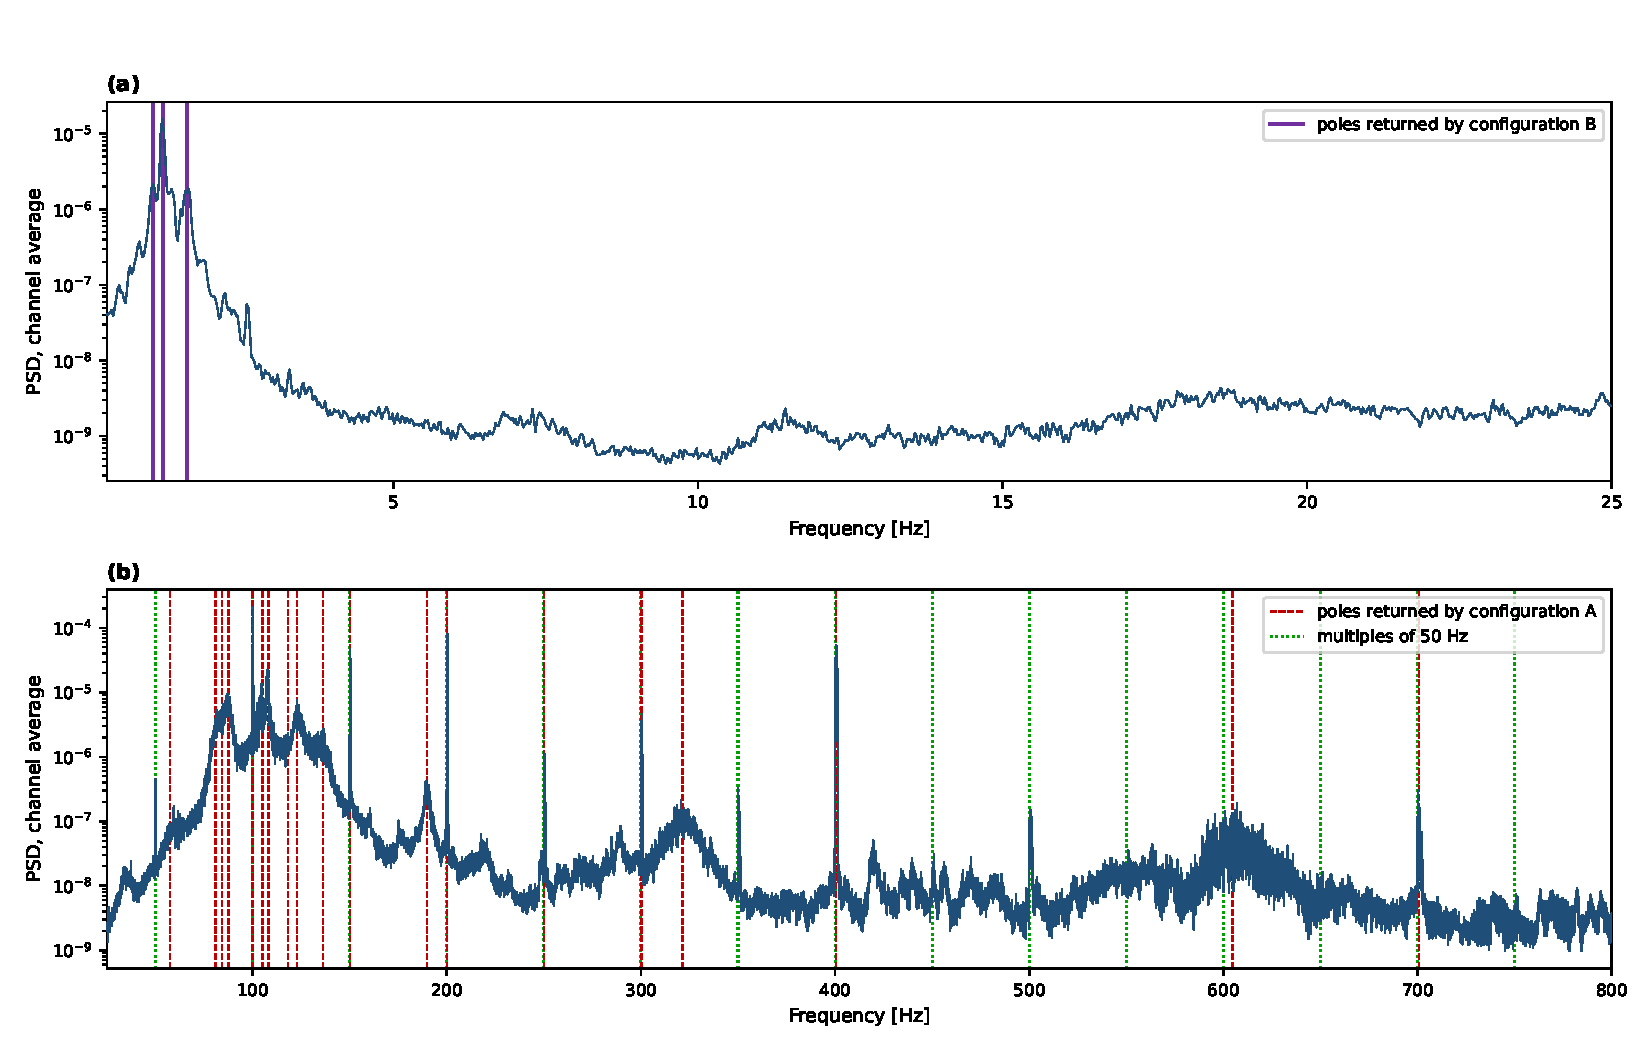
\includegraphics[width=0.95\linewidth]{fig10_configurations}
\caption{The same record seen by configurations A and B of Table~\ref{tab:config}, over (a) the structural band from 0.3 to 25~Hz and (b) the band from 25 to 800~Hz from which configuration A draws its poles. Dotted lines mark multiples of 50~Hz}
\label{fig:harm}
\end{figure}

Seven of the poles returned at the full rate have damping between 0.007 and
0.042\,\%, far below the 0.1\,\% bound of the third check. All seven lie within
0.2\,\% of a multiple of 50~Hz, at 100.17, 150.30, 200.28, 250.26, 300.49,
400.69 and 700.93~Hz. They are harmonics of the mains supply. The other
thirteen poles of configuration A were not classified, since that
configuration is not used.

% =====================================================================
\section{Search for a tower mode below 0.5~Hz}
\label{sec:s-lowband}

The band below 0.5~Hz was searched for a tower mode, which a soft--stiff design
places near 0.3~Hz \cite{arany2017}. The records were decimated further to
12.9~Hz and analysed with a covariance window of 11.6~s
(Figure~\ref{fig:lowband}). Four of the seven records were searched: the
vertical setup and lateral setup 1 of campaign 1, and the lateral setup and
vertical setup d2ke of campaign 2. No pole below 0.5~Hz passes the checks. The only
features are spectral peaks near 0.21~Hz in campaign 1, recorded before the
tower stood and consistent with waves, and near 0.32~Hz in campaign 2, where
the first tower mode is expected.

\begin{figure}[htbp]
\centering
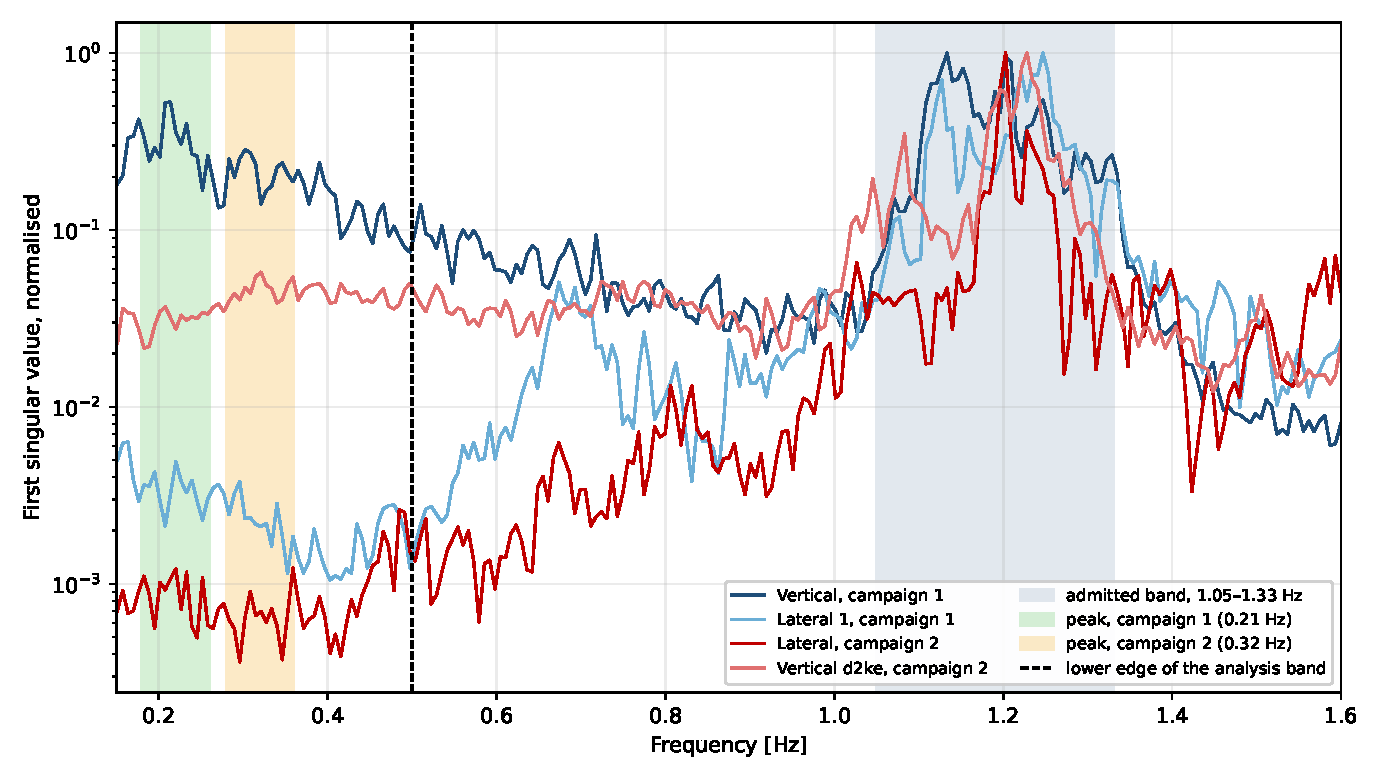
\includegraphics[width=0.85\linewidth]{fig12_low_band}
\caption{Search below the analysis band, with the records decimated to 12.9~Hz and a covariance window of 11.6~s. The only features below 0.5~Hz are the peaks marked at 0.21~Hz in campaign 1 and 0.32~Hz in campaign 2. The first, recorded before the tower stood, is consistent with wave excitation; the second lies where the first tower mode is expected. Neither yields a stable pole}
\label{fig:lowband}
\end{figure}

% =====================================================================
\section{Setup-by-setup comparison of the two campaigns}
\label{sec:s-shift}

Table~\ref{tab:shift} lists the low-band poles behind Figure~9 of the main
paper. Averaging all setups of each campaign suggests a fall of 8.4\,\% after
the tower was installed, but this mixes setups that measure in different
directions and therefore weight different members of the band. The table
compares setups that measure in the same direction.

The differences between setup means hide a larger scatter. Pole by pole, the
three poles of vertical setup d2ke differ from the single pole of the vertical
setup of campaign 1 by $-8.5$, $+2.1$ and $+4.9$\,\%, and the 1.215~Hz pole of
campaign 2 differs from the two poles of lateral setup 1 by $-0.9$ and
$-3.1$\,\%. Between the three segments of one record a pole moves by up to
5\,\% (vertical setup d1: 1.163 and 1.104~Hz, with no pole in the third
segment). The spectral peaks (Table~\ref{tab:poles}) differ from the subspace
poles by up to 5\,\% and, in the vertical setups, rise from campaign 1 to
campaign 2 (1.134 to 1.210 and 1.235~Hz) where the subspace poles fall. The
sign of any change is therefore not determined.

\paragraph{Orientation of channel 4 in campaign 1.} The channel orientations
of the lateral setups of campaign 1 are not recorded. In lateral setup 1 the
amplitude of channel 4 is 0.71 of the mean of the other channels, with a
coherence of 0.94. This is what a fifth horizontal channel would give, and the
setup is treated as horizontal throughout; it is not used for the ratio of
vertical to horizontal motion.

\begin{table}[htbp]
\centering
\caption{Low-band poles by setup, grouped by measured direction, and the change between campaigns for like-for-like setups. V: all channels vertical; H: horizontal, with channel 4 vertical in campaign 2; M: one vertical and two horizontal channels}
\label{tab:shift}
\begin{tabular}{@{}ccllr@{}}
\toprule
Dir. & Camp. & Setup & Poles (Hz) & Setup mean (Hz) \\
\midrule
V & 1 & Vertical & 1.174 & 1.174 \\
V & 2 & Vertical d1 & 1.147 & 1.147 \\
V & 2 & Vertical d2ke & 1.074, 1.199, 1.231 & 1.168 \\
  &   & \multicolumn{3}{l}{change, vertical: $-2.3$\,\% and $-0.5$\,\%} \\
\midrule
H & 1 & Lateral 1 & 1.226, 1.254 & 1.240 \\
H & 1 & Lateral 2 & 1.322 & 1.322 \\
H & 2 & Lateral & 1.052, 1.215 & 1.134 \\
  &   & \multicolumn{3}{l}{change, 1.215~Hz pole against lateral 1: $-2.0$\,\%} \\
\midrule
M & 1 & Three-channel & 1.238, 1.331 & 1.284 \\
\bottomrule
\end{tabular}
\end{table}

\begin{thebibliography}{9}

\bibitem{arany2017}
Arany L, Bhattacharya S, Macdonald J, Hogan SJ (2017) Design of monopiles for offshore wind turbines in 10 steps. Soil Dynamics and Earthquake Engineering 92:126--152. \url{https://doi.org/10.1016/j.soildyn.2016.09.024}

\end{thebibliography}

\end{document}
